\documentclass[10pt,twocolumn,a4paper]{article}
\usepackage[utf8]{inputenc}
\usepackage[spanish,es-nodecimaldot]{babel}
\usepackage[margin=1.50cm, top=1.45cm, bottom=1.55cm]{geometry}
\usepackage{graphicx}
\usepackage{booktabs}
\usepackage{amsmath,amssymb}
\usepackage{microtype}
\usepackage{caption}
\usepackage{titlesec}
\usepackage{tabularx}
\usepackage{xurl}
\usepackage[hidelinks]{hyperref}

% Configuracion de directorios de graficos para Overleaf y compiladores locales
\graphicspath{{figures/}{./}}

% Control tipografico estricto de espaciados entre encabezados y texto
\titlespacing*{\section}{0pt}{4.8pt plus 1pt minus 1pt}{1.8pt plus 0.5pt minus 0.5pt}
\titlespacing*{\subsection}{0pt}{3.2pt plus 0.8pt minus 0.8pt}{1.2pt plus 0.4pt minus 0.4pt}
\captionsetup{font=small,labelfont=bf,labelsep=period,skip=3pt}
\setlength{\textfloatsep}{6pt plus 1pt minus 1pt}
\setlength{\dbltextfloatsep}{7pt plus 1pt minus 1pt}
\setlength{\floatsep}{5pt plus 1pt minus 1pt}
\setlength{\dblfloatsep}{5pt plus 1pt minus 1pt}
\renewcommand{\dbltopfraction}{0.90}
\renewcommand{\topfraction}{0.90}
\renewcommand{\textfraction}{0.08}
\renewcommand{\floatpagefraction}{0.85}

% Comando formal de sangria francesa para referencias estilo APA 7
\newcommand{\apabibentry}[1]{\noindent\hangindent=0.6cm\hangafter=1 #1\vspace{0.25cm}\par}

\title{\vspace{-0.85cm}\textbf{\Large Evaluación Diagnóstica de la Separabilidad Espacial en el Rift de Baja California: Alcances y Limitaciones del Aprendizaje Automático Regional}}
\author{\textbf{Rubén Rivera García}\\
\small Departamento de Ciencias de la Computación, Centro de Investigación Científica y de Educación Superior de Ensenada (CICESE)\\
\small Asignatura. Ciencia de Datos (Semestre 2026-3) -- Profesor. Dr. Irvin Hussein López Nava}
\date{Noviembre de 2026\vspace{-0.45cm}}

\begin{document}

\maketitle

\begin{abstract}
\noindent La aplicación del aprendizaje automático a la exploración geotérmica enfrenta un riesgo metodológico importante: que la correlación espacial, la cobertura superficial de origen antrópico y las discontinuidades cartográficas se interpreten erróneamente como señales físicas del subsuelo. Este trabajo presenta un estudio diagnóstico y reproducible que evalúa en qué medida covariables estructurales, magnéticas y morfológicas de acceso público permiten distinguir el polígono del campo de Cerro Prieto de zonas de fondo con dificultad creciente en el Valle de Mexicali. Se analizaron 89,815 celdas georreferenciadas de 30~m, cuya prevalencia de clase positiva (27.6\%) es resultado deliberado del diseño muestral y no de la prevalencia regional real (aproximadamente 0.075\%). Se contrastaron una partición aleatoria convencional (Protocolo A) y una validación cruzada en cinco pliegues espaciales con zona de exclusión de 500~m (Protocolo B). Con la partición aleatoria, los modelos no lineales alcanzan un PR-AUC superior a 0.999; bajo validación espacial, el PR-AUC medio se ubica entre 0.9527 y 0.9624 con notable incremento de varianza. La regresión logística con dos descriptores heurísticos ($R_{TE}, I_{TT}$) obtiene un desempeño comparable al de Random Forest y al del perceptrón multicapa (MLP), con menor dispersión inter-pliegues ($\pm 0.0398$ frente a $\pm 0.0686$ y $\pm 0.0702$) y mejor calibración de Brier (0.04862 frente a 0.06492 y 0.06652). El umbral óptimo de Youden en el MLP exhibe una severa inestabilidad espacial (rango de 0.8857). Asimismo, un modelo basado exclusivamente en coordenadas geográficas alcanza, en el Pliegue 5, un PR-AUC similar al de los modelos multivariados completos, mientras que placebos sintéticos de fallas desplazadas igualan o superan a las trazas reales. En la cartografía regional acotada por el Área de Aplicabilidad (AOA), el sector de El Chinero, señalado antes como prospecto ciego, obtiene una puntuación mediana de apenas 0.03326 en el modelo multivariado (y 0.00387 sin variables superficiales), demostrando que su valor previo derivaba de un sesgo posicional del mapa de fallas.
\end{abstract}

\section{Introducción y Planteamiento del Problema}
En la cuenca pull-apart del Valle de Mexicali, el Campo Geotérmico de Cerro Prieto constituye el único complejo comercial en operación y, por lo tanto, la única fuente de celdas positivas comprobadas de la región (Elders et al., 1984). Esta condición impone una restricción epistemológica mayor: un algoritmo supervisado puede optimizarse memorizando la fisiografía local, la infraestructura industrial de la central o los contrastes de la cartografía, en lugar de aprender regularidades hidrotermales generalizables a sectores no explorados (\textit{single-field problem}).

La temperatura superficial terrestre (LST) diurna captada por satélite está dominada por la insolación solar pasiva del desierto. Por su parte, la distancia a trazas de falla y la magnetometría aerotransportada suelen emplearse bajo el supuesto de que representan, de forma directa, permeabilidad activa y desmagnetización térmica profunda. Sin embargo, en ausencia de una validación espacial rigurosa que neutralice la autocorrelación (Roberts et al., 2017; Ploton et al., 2020), resulta imposible dilucidar cuánta de la capacidad predictiva proviene de procesos termodinámicos endógenos y cuánta de tendencias espaciales sistemáticas de la cuenca.

Para abordar este problema se formularon tres preguntas de investigación formales. Primera ($PI_1$): qué tan separable es el polígono de Cerro Prieto frente a fondos regionales de dificultad creciente (B1: 0.5--2~km; B2: 2--5~km; B3: $>$5~km) y qué fracciona el acoplamiento físico frente a la posición. Segunda ($PI_2$): cuantificar el impacto de sustituir la partición aleatoria ingenua por una validación cruzada en bloques espaciales con zona de exclusión de 500~m. Tercera ($PI_3$): verificar si clasificadores no lineales complejos (Random Forest y MLP) superan a un modelo lineal con términos de interacción en capacidad discriminativa, calibración probabilística (Brier score) y estabilidad de umbrales operativos de decisión.

\section{Covariables, Insumos Cartográficos y Muestreo}
El espacio muestral integra 89,815 celdas de 30~m en coordenadas UTM Zona 11N (Datum WGS84). Se procesaron seis covariables físicas primarias (elevación, pendiente, LST, NDVI, distancia a fallas y magnetometría) y dos descriptores heurísticos combinados. La elevación y pendiente provienen del Continuo de Elevaciones Mexicano (CEM 3.0) del INEGI; la LST y el índice de vegetación (NDVI) se extrajeron de escenas Landsat 9 (sensores TIRS-2 y OLI-2) en condiciones estivales despejadas.

\begin{figure}[htbp]
\centering
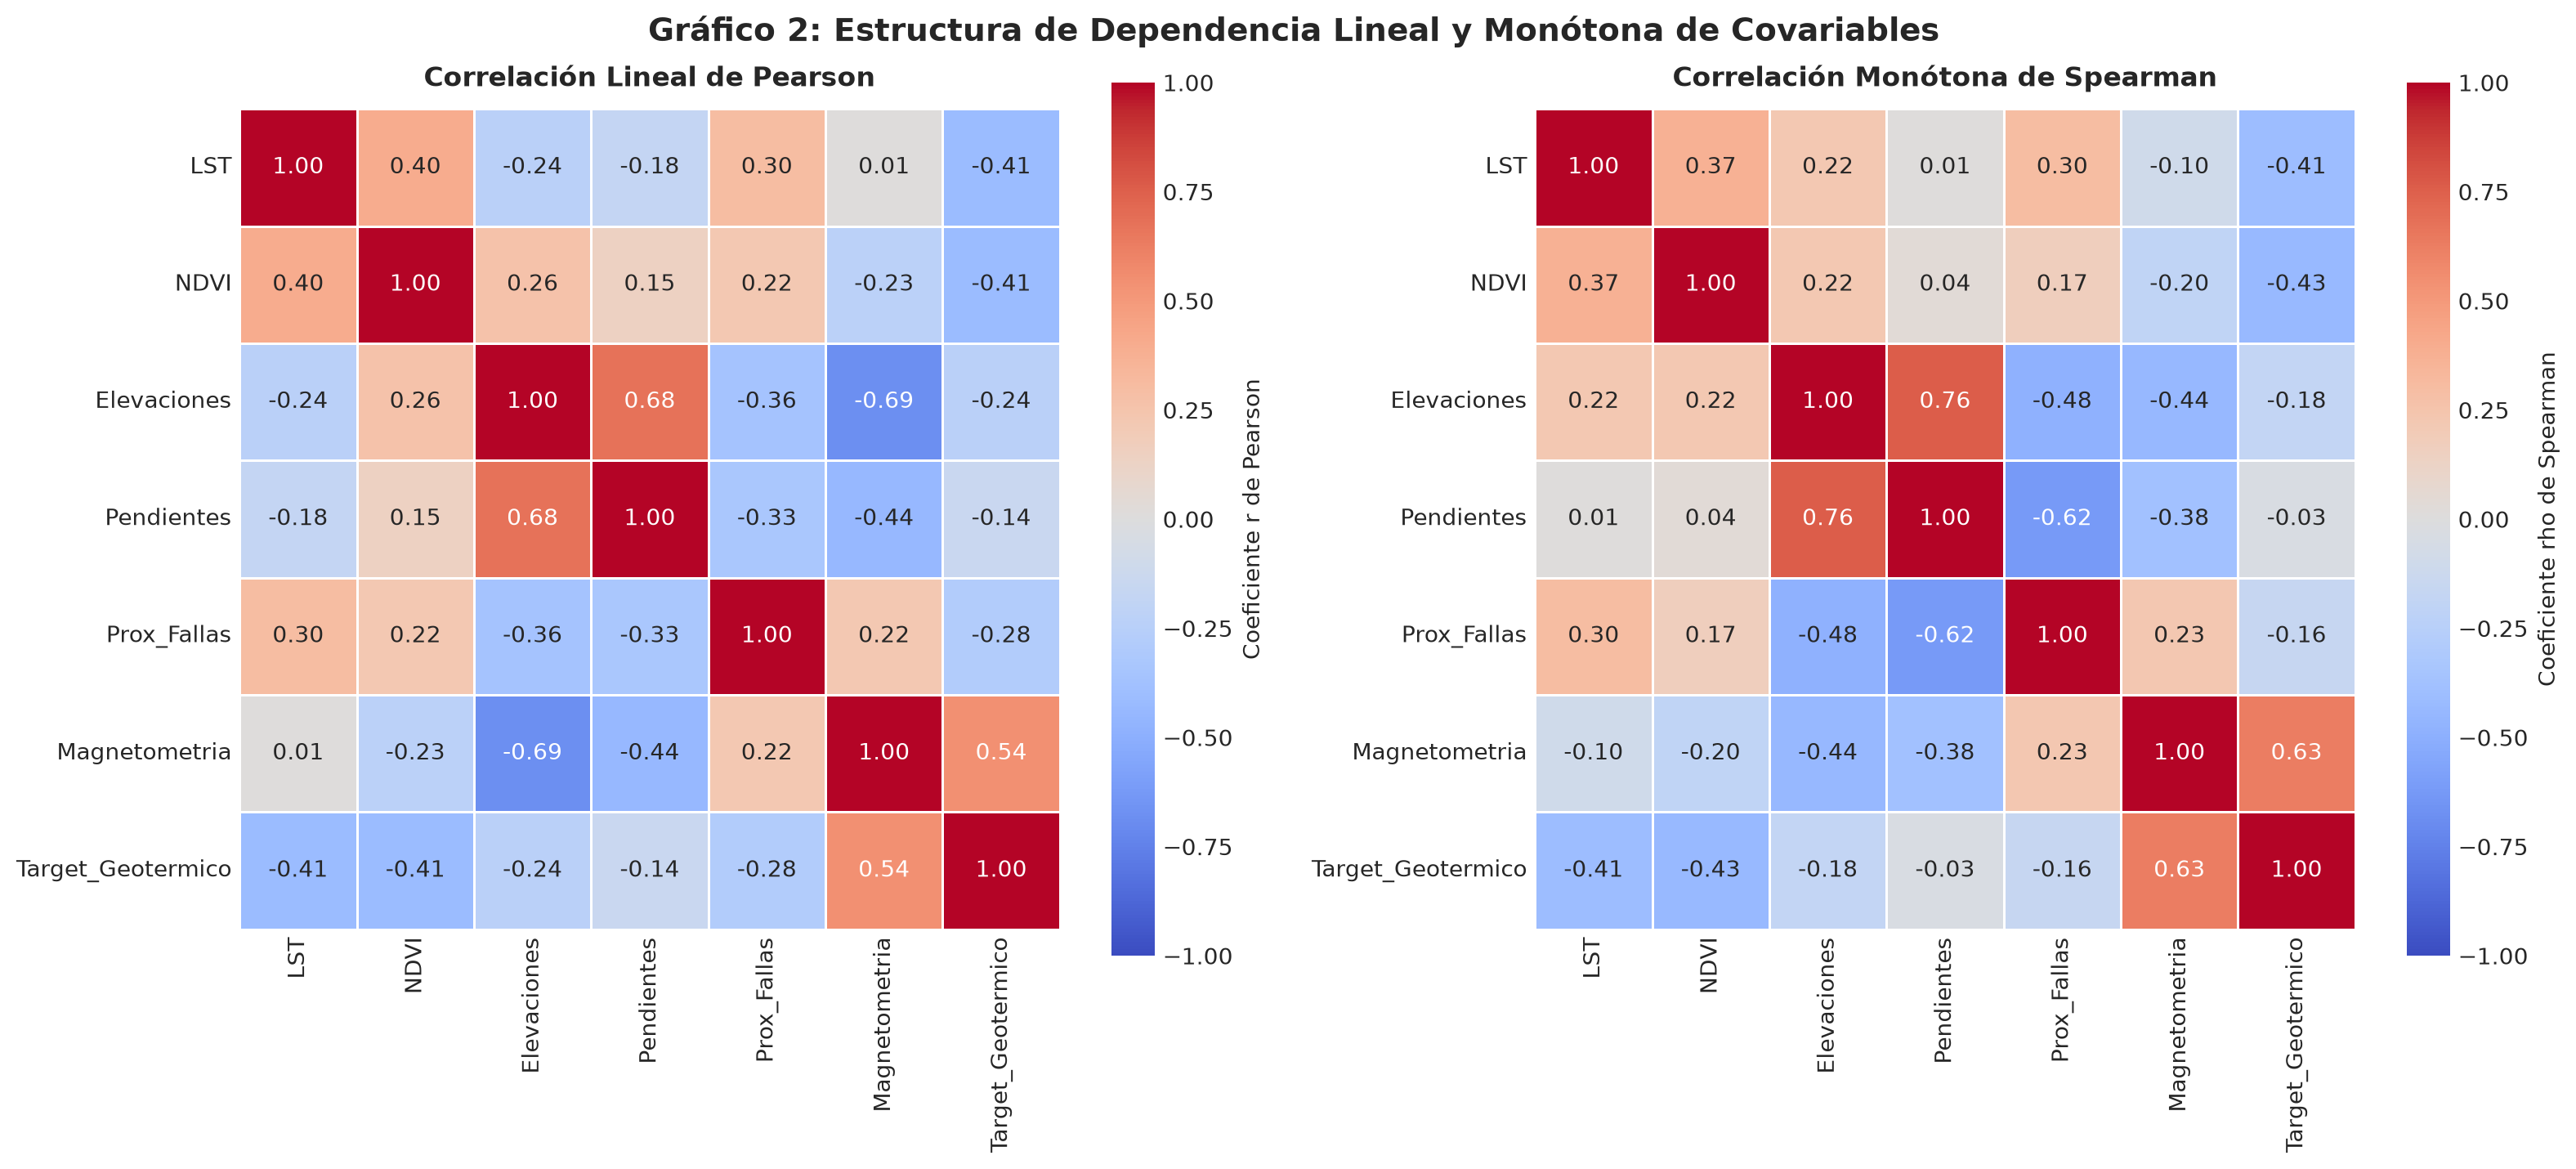
\includegraphics[width=\columnwidth]{grafico_2_matriz_correlacion.png}
\caption{Matriz de correlación bivariada entre covariables físicas primarias y pertenencia a la clase positiva.}
\label{fig2}
\end{figure}

Como resume la matriz de correlación bivariada de la Figura~\ref{fig2}, las covariables morfológicas y térmicas presentan distintos grados de asociación lineal con el objetivo. Para la estructura tectónica se digitalizaron las fallas de las cartas geológico-mineras del Servicio Geológico Mexicano (SGM, 2020), reproyectadas de NAD27 a WGS84 mediante transformación geodésica estándar (desplazamiento medio medido de 197.8~m). Sobre ellas se computó la distancia euclidiana hacia la traza más próxima (\texttt{dist\_fallas\_SGM\_m}). El campo magnético se obtuvo del mosaico aeromagnético continuo (\texttt{Magnetometria}), en nanoteslas (nT).

Con el propósito de linealizar interacciones no lineales directas, se construyeron dos descriptores heurísticos: el Ratio Termo-Estructural ($R_{TE}$) y el Índice Topo-Térmico ($I_{TT}$):
\begin{equation}
R_{TE} = \frac{\mathrm{LST}}{\ln(d + 10.0)}
\label{eq_rte}
\end{equation}
\begin{equation}
I_{TT} = \frac{\mathrm{LST}}{z + 50.0}
\label{eq_itt}
\end{equation}
donde $d$ denota la distancia euclidiana en metros a la falla más cercana y $z$ representa la cota topográfica en m.s.n.m. Los escalares de 10~m y 50~m previenen indeterminaciones analíticas. Constituyen aproximaciones de ingeniería y no leyes termodinámicas fundamentales.

El muestreo es biestratificado. La clase positiva comprende el censo íntegro del polígono concesionado de Cerro Prieto ($N_1 = 24,814$ celdas). Los negativos ($N_0 = 65,001$ celdas) se distribuyeron equitativamente (21,667 por estrato) en tres coronas concéntricas: B1 (0.5 a 2~km), B2 (2 a 5~km) y B3 ($>$5~km), excluyendo un buffer de seguridad de 0 a 500~m. La prevalencia del dataset (27.6\%) responde a una conveniencia computacional y no a la prevalencia regional real del fenómeno, estimada en $\approx 0.075\%$ (22.33~km$^2$ de campo sobre 29,758~km$^2$ de dominio analizado).

\begin{table*}[t]
\centering
\caption{Comparativa cuantitativa bajo partición aleatoria (Protocolo A, $N_{\text{test}} = 13,473$) frente a validación cruzada en 5 pliegues espaciales con buffer de exclusión de 500~m (Protocolo B).}
\label{tab1}
\footnotesize
\setlength{\tabcolsep}{4.2pt}
\begin{tabular}{lcccccc}
\toprule
 & \multicolumn{3}{c}{\textbf{Protocolo A (Partición Aleatoria)}} & \multicolumn{3}{c}{\textbf{Protocolo B (Validación Espacial 5P)}} \\
\cmidrule(lr){2-4} \cmidrule(lr){5-7}
\textbf{Modelo} & \textbf{ROC-AUC} & \textbf{PR-AUC} & \textbf{Brier Score} & \textbf{ROC-AUC} & \textbf{PR-AUC} & \textbf{Brier Score} \\
\midrule
Clasificador Base Dummy & 0.5000 & 0.2763 & 0.19997 & 0.5000 $\pm$ 0.0000 & 0.3068 $\pm$ 0.1030 & 0.22101 $\pm$ 0.04901 \\
Regresión Logística (con $R_{TE}, I_{TT}$) & 0.9894 & 0.9732 & 0.03744 & 0.9819 $\pm$ 0.0166 & 0.9527 $\pm$ 0.0398 & 0.04862 $\pm$ 0.02775 \\
Random Forest (100 árboles) & 1.0000 & 0.9999 & 0.00362 & 0.9785 $\pm$ 0.0363 & 0.9555 $\pm$ 0.0686 & 0.06492 $\pm$ 0.07326 \\
MLP PyTorch (Ensamble 3 semillas) & 0.9999 & 0.9997 & 0.00391 & 0.9758 $\pm$ 0.0504 & 0.9624 $\pm$ 0.0702 & 0.06652 $\pm$ 0.09103 \\
\bottomrule
\end{tabular}
\end{table*}

\section{Metodología y Diseño de Evaluación}
Para evitar cualquier fuga de información (*data leakage*), el escalador estándar (\texttt{StandardScaler}) se ajustó única y exclusivamente con los datos de entrenamiento de cada pliegue. Se prescindió formalmente de técnicas de sobremuestreo sintético (\texttt{SMOTE}) para no generar vectores artificiales interpolados en regiones geográficas no muestreadas, y no se aplicaron ponderaciones de pérdida (\texttt{pos\_weight}), preservando la calibración probabilística natural.

El Protocolo A aplica una división estratificada celda a celda (70/15/15). El Protocolo B fragmenta el polígono de Cerro Prieto en cinco sectores geográficos contiguos dispuestos de norte a sur. En cada iteración, un sector se mantiene como prueba ciega y se aplica una franja de exclusión de 500~m en su perímetro, suprimiendo la transferencia espuria por contigüidad espacial inmediata.

Se evaluaron tres familias algorítmicas bajo semillas deterministas:
\begin{enumerate}
\itemsep0pt \parsep0pt \topsep1.5pt
\item \textbf{Regresión Logística:} optimizador L-BFGS con penalización $L_2$ ($C = 1.0$), entrenada sobre las ocho covariables normalizadas.
\item \textbf{Random Forest:} ensamble de 100 árboles con profundidad máxima de 12 niveles; se promediaron las probabilidades de tres semillas pseudoaleatorias (42, 43 y 44).
\item \textbf{Perceptrón Multicapa (MLP):} red neuronal en PyTorch con topología 8-64-64-32-1, no linealidad LeakyReLU ($\alpha = 0.25$; He et al., 2015), normalización por lotes (\texttt{BatchNorm1d}), desconexión aleatoria (\texttt{Dropout(0.10)}) y optimizador AdamW (tasa $\eta = 0.001$, decaimiento $\lambda = 10^{-4}$, 15 épocas en ensamble espacial y 25 en Protocolo A). El ensamble integra el promedio de logits de tres inicializaciones.
\end{enumerate}

Las métricas cuantitativas comprenden ROC-AUC, PR-AUC y el error cuadrático medio de Brier. Los umbrales de corte se optimizaron mediante el índice de Youden ($J = \text{Sensibilidad} + \text{Especificidad} - 1$) evaluado sobre el entrenamiento de cada pliegue. Adicionalmente, se delimitó la validez territorial con el Área de Aplicabilidad (AOA) de Meyer y Pebesma (2021) calculando el Índice de Disimilitud (DI) ponderado por importancia de permutación. El código fuente, scripts de reproducibilidad y datos curados se encuentran disponibles en: \url{https://github.com/rubenriv2111-beep/ICD-2026}.

\section{Resultados y Diagnósticos Experimentales}

\subsection{Partición Aleatoria frente a Validación Espacial}
Bajo partición aleatoria (Protocolo A), los modelos no lineales exhiben puntuaciones casi perfectas con ROC-AUC y PR-AUC $\ge 0.999$ y Brier $< 0.004$ (Cuadro \ref{tab1}). Sin embargo, bajo validación espacial por bloques (Protocolo B), el PR-AUC medio desciende a un intervalo de 0.9527 a 0.9624, incrementándose significativamente la dispersión. Las divergencias entre modelos en el Protocolo B resultan inferiores a 0.01 en PR-AUC y quedan comprendidas dentro de las desviaciones estándar inter-pliegues, desestimando la superioridad categórica de las arquitecturas no lineales complejas.

El Cuadro \ref{tab2} evidencia un rendimiento elevado y estable en los pliegues septentrionales y centrales (1 al 4), donde Random Forest y el MLP alcanzan PR-AUC entre 0.9716 y 1.0000. No obstante, el desempeño colapsa en el Pliegue 5 (extremo sur de Cerro Prieto): Random Forest y el MLP caen a PR-AUC de 0.8352 y 0.8381, disparándose el Brier del MLP a 0.22314. En contraposición, la Regresión Logística sostiene un PR-AUC de 0.91486 y Brier de 0.09519. En promedio global, el modelo lineal con interacciones supera a Random Forest en ROC-AUC (0.9819 frente a 0.9785) y Brier (0.04862 frente a 0.06492) con una varianza sustancialmente menor ($\pm 0.0166$ vs. $\pm 0.0363$).

\begin{table}[htbp]
\centering
\caption{Desempeño por pliegue bajo el Protocolo B (Buffer 500~m).}
\label{tab2}
\resizebox{\columnwidth}{!}{%
\begin{tabular}{clcccc}
\toprule
\textbf{Pliegue} & \textbf{Modelo} & \textbf{ROC-AUC} & \textbf{PR-AUC} & \textbf{Brier} & \textbf{Umbral $J$} \\
\midrule
1 & Regr. Logística & 0.9930 & 0.9687 & 0.0321 & 0.2458 \\
  & Random Forest    & 0.9868 & 0.9725 & 0.0576 & 0.4488 \\
  & MLP Ensamble     & 0.9994 & 0.9983 & 0.0143 & 0.7346 \\
\midrule
2 & Regr. Logística & 0.9925 & 0.9860 & 0.0317 & 0.4072 \\
  & Random Forest    & 0.9989 & 0.9982 & 0.0211 & 0.1279 \\
  & MLP Ensamble     & 0.9993 & 0.9990 & 0.0130 & 0.0165 \\
\midrule
3 & Regr. Logística & 0.9951 & 0.9886 & 0.0305 & 0.3801 \\
  & Random Forest    & 1.0000 & 1.0000 & 0.0043 & 0.1801 \\
  & MLP Ensamble     & 1.0000 & 1.0000 & 0.0117 & 0.2182 \\
\midrule
4 & Regr. Logística & 0.9711 & 0.9053 & 0.0536 & 0.1652 \\
  & Random Forest    & 0.9923 & 0.9716 & 0.0516 & 0.1297 \\
  & MLP Ensamble     & 0.9945 & 0.9768 & 0.0705 & 0.0895 \\
\midrule
5 & Regr. Logística & 0.9579 & 0.9149 & 0.0952 & 0.3540 \\
  & Random Forest    & 0.9143 & 0.8352 & 0.1900 & 0.3522 \\
  & MLP Ensamble     & 0.8856 & 0.8381 & 0.2231 & 0.9022 \\
\bottomrule
\end{tabular}%
}
\end{table}

\subsection{Variabilidad del Umbral de Decisión en el MLP}
El umbral de Youden ($J$) exhibe una dispersión severa e inestable en el MLP a lo largo de los pliegues espaciales: oscila desde 0.0165 en el Pliegue 2 hasta 0.9022 en el Pliegue 5, cubriendo un rango de 0.8857. En Random Forest, la cota oscila en un rango más restringido de 0.3209 (0.1279 a 0.4488). Este fenómeno certifica que los logits neuronales distorsionan su escala absoluta entre subdominios espaciales, invalidando el empleo de umbrales rígidos fijos ($F_1$, precisión o sensibilidad a corte 0.5) en tareas de inferencia regional sin recalibración local previa. La Figura~\ref{fig6} corrobora este comportamiento al contrastar las curvas ROC en escala logarítmica de falsas alarmas, donde los tres clasificadores exhiben separaciones operativas diferenciadas en el rango de alta especificidad.

\begin{figure}[htbp]
\centering
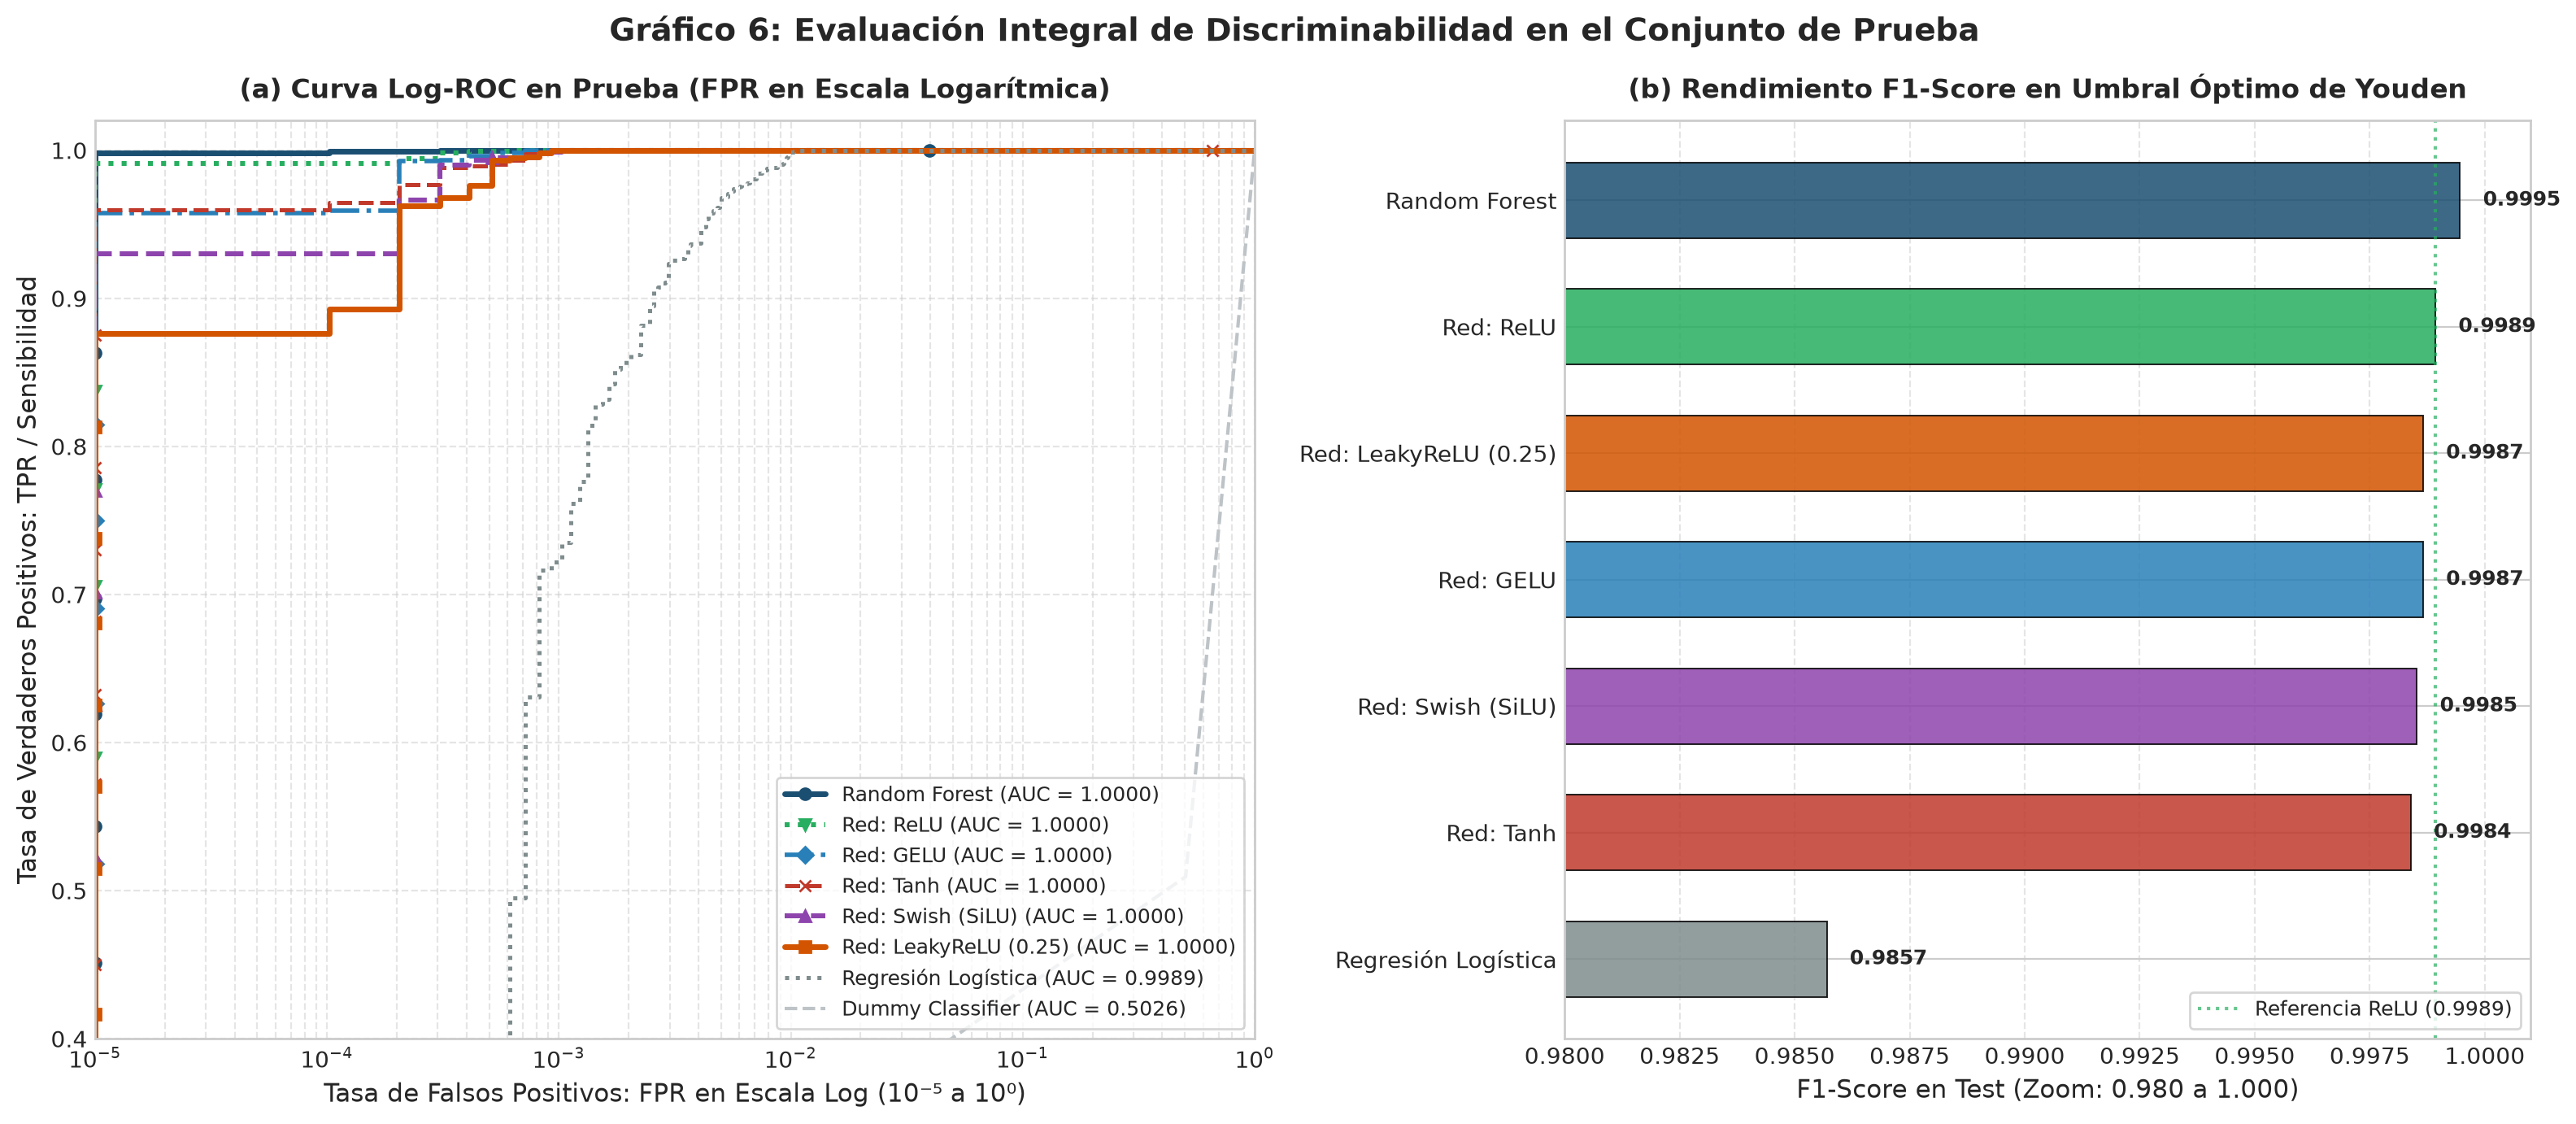
\includegraphics[width=\columnwidth]{grafico_6_curvas_roc_comparativas.png}
\caption{Curvas ROC en escala logarítmica de falsas alarmas para el conjunto de prueba independiente.}
\label{fig6}
\end{figure}

\subsection{Diagnóstico Posicional con Coordenadas Solas}
\label{sec:pos}
Para dilucidar si la separabilidad se explica exclusivamente por la ubicación espacial, se ajustó un modelo Random Forest alimentado únicamente con coordenadas UTM ($x_{\text{utm}}, y_{\text{utm}}$). En el Pliegue 5, este clasificador posicional alcanza un ROC-AUC de 0.94718 y PR-AUC de 0.84255 frente a una prevalencia basal de 0.36116. Dicho valor iguala el PR-AUC obtenido por Random Forest (0.8352) y el MLP (0.8381) utilizando las ocho covariables geofísicas. Más aún, frente a los estratos B2 (2--5~km) y B3 ($>$5~km), las coordenadas solas obtienen ROC-AUC y PR-AUC idénticos a 1.00000. Esto demuestra empíricamente que, en las periferias de la cuenca, la clase positiva se segrega primordialmente por su confinamiento geográfico local.

\subsection{Pruebas Dirigidas: Placebos y Cobertura Superficial}
Con el fin de verificar si la distancia a fallas representa permeabilidad hidrotermal o un gradiente posicional genérico, se diseñó un experimento de placebos espaciales desplazando las trazas tectónicas $\pm 10$~km en $x$ e $y$ y rotándolas 90$^\circ$ alrededor del centroide de Cerro Prieto. En el Pliegue 1, el placebo desplazado 10~km al oeste supera a las fallas verdaderas (PR-AUC 0.5978 vs. 0.5916). En el Pliegue 5, el placebo desplazado 10~km al este supera ampliamente a la falla real (PR-AUC 0.89049 frente a 0.64238; ROC-AUC 0.95919 frente a 0.87249). Este resultado revela que la covariable actúa como un proxy de lejanía a los bordes de cuenca y no como un acoplamiento físico reservorio-fractura.

Por otra parte, se cuantificó el sesgo de uso de suelo: el 49.15\% de los positivos de Cerro Prieto (12,195 celdas) presenta firmas espectrales de agua y humedad anómala ($\text{MNDWI} > 0 \lor \text{NDVI} < 0$), coincidentes con las lagunas de evaporación, salmueras y pozos de inyección de la central activa. En el Pliegue 5, donde la humedad antrópica desciende al 12.03\%, un modelo basado exclusivamente en firmas superficiales colapsa a PR-AUC de 0.52110. Al evaluar únicamente el subconjunto de celdas positivas secas (50.85\% del yacimiento), el modelo multivariado retiene un PR-AUC de 0.92729, demostrando que logra apoyarse en la morfología estructural cuando cesa la signatura artificial del agua superficial.

\subsection{Artefacto Cartográfico en la Magnetometría Regional}
\label{sec:mag}
Al aislar la magnetometría residual, su capacidad discriminativa aparente crece en función de la distancia geográfica: ROC-AUC de 0.63912 frente a la Banda 1 (distancia mediana de 1,274~m), 0.64413 frente a la Banda 2 (3,600~m) y 0.98321 frente a la Banda 3 en la llanura de San Felipe (92,760~m). No obstante, el 69.45\% de las celdas válidas de la hoja San Felipe H11-3 presenta un gradiente horizontal exactamente nulo (0~nT/30~m), en contraste con el 35.81\% en la hoja Mexicali H11-12. Esta meseta de gradiente cero confirma una costura cartográfica derivada de métodos de digitalización dispares entre épocas, advirtiendo que la separabilidad lejana responde a una discontinuidad del insumo y no a termodesmagnetización profunda.

\begin{figure*}[t]
\centering
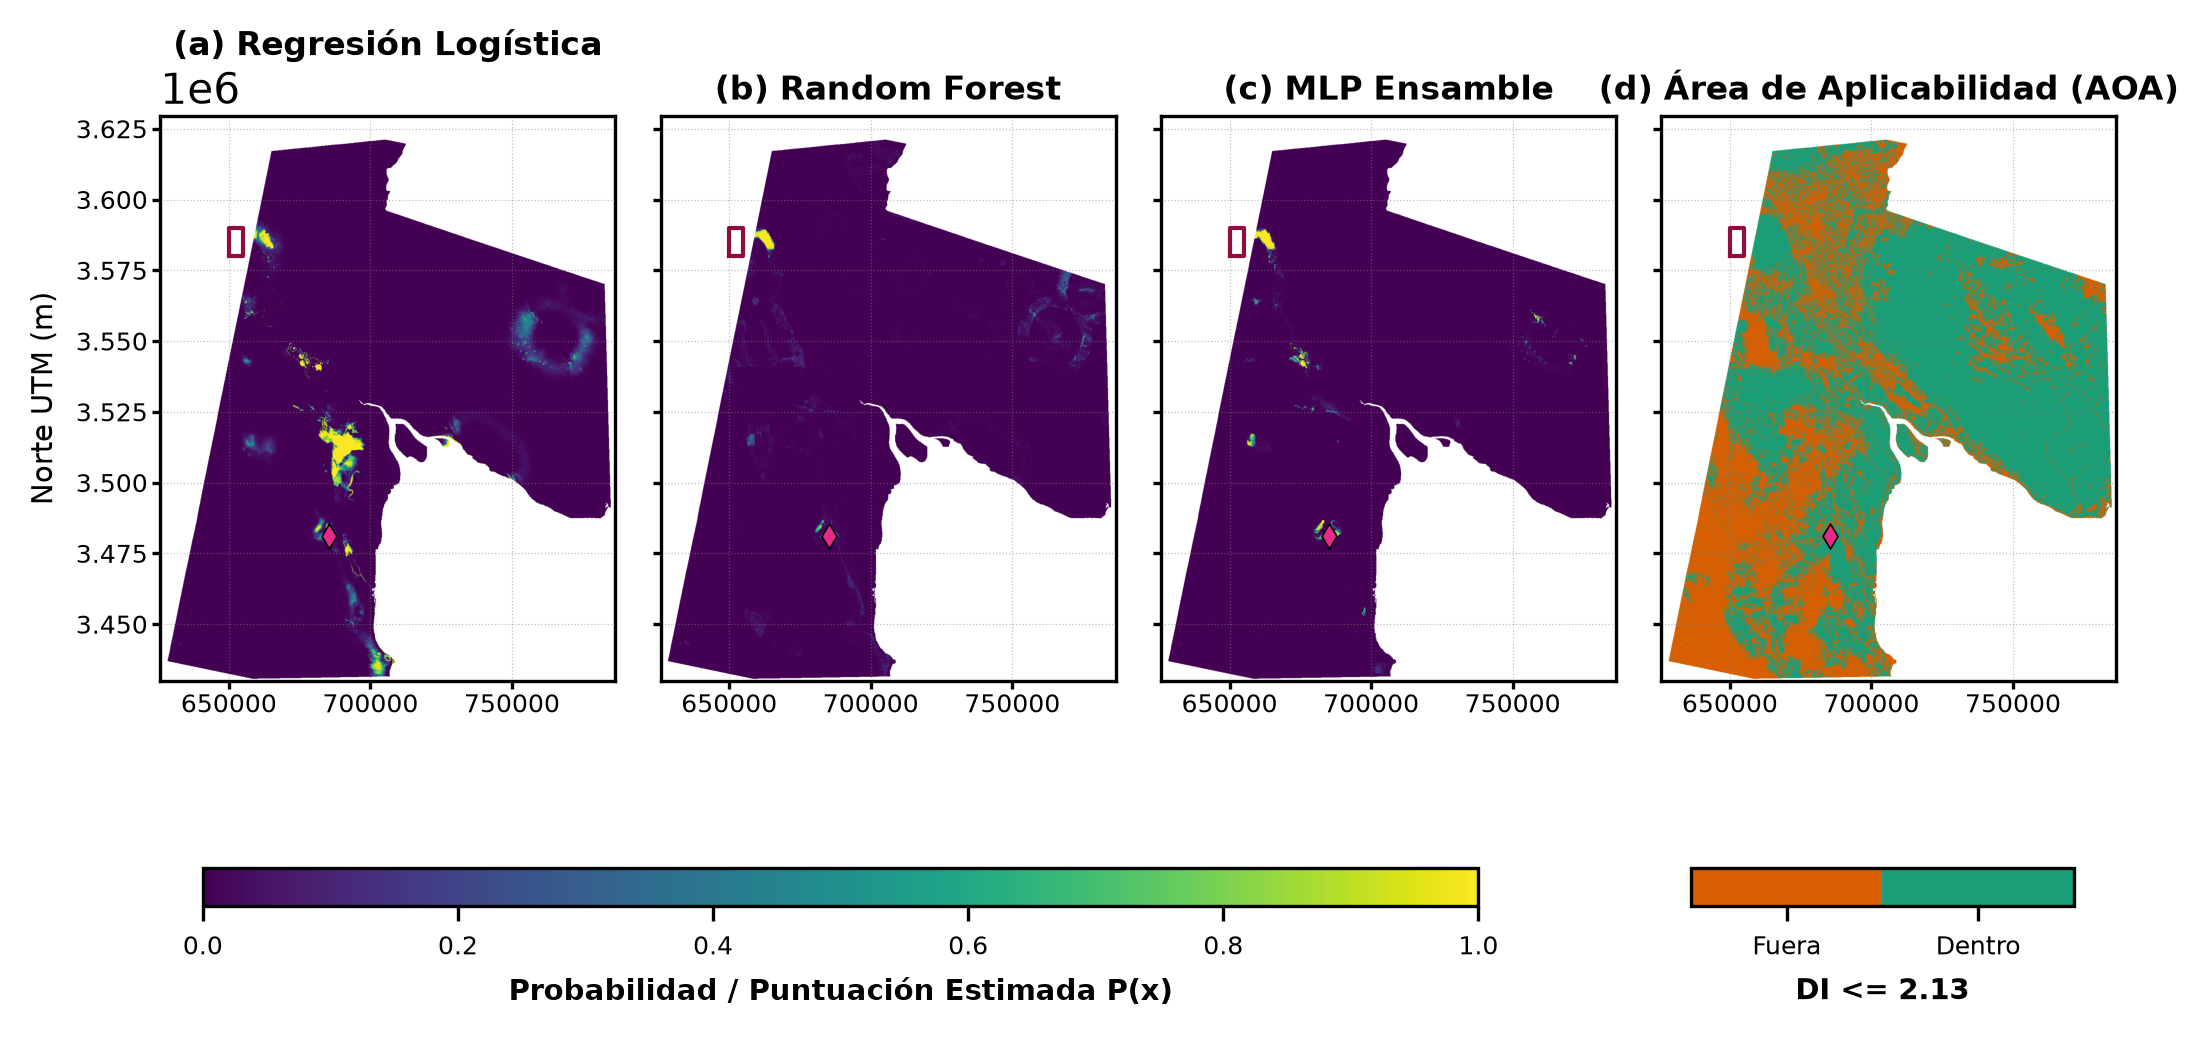
\includegraphics[width=\textwidth]{grafico_10_mapa_susceptibilidad_espacial.png}
\caption{Cartografía de inferencia exploratoria regional multimodelo sobre la rejilla continua de 120~m proyectada en tira horizontal estándar de dos columnas IEEE (ancho de 180~mm a 300~DPI). Paneles: (a) Regresión Logística con descriptores heurísticos ($R_{TE}, I_{TT}$), (b) Random Forest (100 árboles), (c) MLP Ensamble (3 semillas, LeakyReLU $\alpha = 0.25$) compartiendo una barra continua de probabilidad estimada $P(x) \in [0, 1]$, y (d) Área de Aplicabilidad (AOA de Meyer y Pebesma) delimitada por el Índice de Disimilitud ponderado ($\text{DI} \le 2.13$). El polígono en rojo delimita Cerro Prieto; la flecha magenta señala El Chinero, cuya baja puntuación multivariada (mediana 0.03326) y ubicación fuera del AOA en su punto central descartan su viabilidad como prospecto ciego.}
\label{fig10}
\end{figure*}

\section{Discusión y Reevaluación Regional}

\subsection{Acoplamiento Tectónico frente a Gradiente Posicional}
Los contrastes entre partición aleatoria y validación espacial imponen una reinterpretación objetiva. Bajo bloques geográficos, la regresión logística con descriptores de interacción iguala o supera a Random Forest y al MLP, logrando en el Pliegue 5 un PR-AUC de 0.915 frente al 0.843 del clasificador de coordenadas puras. Esto prueba que las variables físicas aportan señal complementaria a la posición. Sin embargo, la sustitución ventajosa de fallas por placebos desplazados confirma que los algoritmos explotan la geometría espacial de la depresión del rift más que leyes hidrogeológicas universales.

\subsection{Reevaluación del Sector El Chinero}
El sector de El Chinero (31.45$^\circ$~N, 115.05$^\circ$~O; UTM 11N: $X = 685,295$~m, $Y = 3,481,120$~m) fue catalogado en exploraciones preliminares basadas exclusivamente en distancias a fallas como un supuesto prospecto ciego con puntuaciones univariadas $>0.90$.

La cartografía regional multivariada de la Figura~\ref{fig10} desmiente categóricamente dicha condición:
\begin{enumerate}
\itemsep0pt \parsep0pt \topsep1.5pt
\item \textbf{Puntuación multivariada:} en los paneles (a, b, c) de la Figura~\ref{fig10}, la puntuación mediana asignada a El Chinero por los modelos multivariados completos es de apenas \textbf{0.03326} (percentil 95 de 0.81977). Al remover las covariables superficiales (LST y NDVI), la mediana colapsa a \textbf{0.00387}.
\item \textbf{Contraste aeromagnético:} la anomalía magnética en El Chinero (mediana de $-225$~nT) se sitúa en el percentil \textbf{0.00\%} respecto a Cerro Prieto (+110 a +350~nT), evidenciando que el algoritmo extrapola sobre una firma física no observada.
\item \textbf{Incertidumbre y AOA:} en el panel (d) de la Figura~\ref{fig10}, el punto central de El Chinero queda catalogado fuera del Área de Aplicabilidad ($\text{DI} > 2.1339$), situándose en una franja de transición geomorfológica donde el 33.79\% del entorno local a 3~km corresponde a extrapolación. Su elevada susceptibilidad aparente inicial respondía al sesgo posicional de las fallas del SGM acoplado a la costura cartográfica del paralelo 32$^\circ$~N.
\end{enumerate}

\subsection{Área de Aplicabilidad (AOA) e Incertidumbre}
En la malla regional continua de 120~m (Figura~\ref{fig10}d), el 62.82\% del dominio territorial permanece dentro del AOA (restringido con coherencia física al fondo sedimentario de la cuenca y valles aluviales, mientras que el 37.18\% restante en sierras graníticas como Cucapá y el sector meridional de San Felipe queda catalogado como extrapolación). No obstante, al inspeccionar el 0.1\% de las celdas con mayores puntuaciones residuales fuera del polígono ($>$5~km), los modelos exhiben discrepancias cualitativas: en Regresión Logística (Figura~\ref{fig10}a) predominan parcelas agrícolas irrigadas del delta ($\text{MNDWI} > 0$), mientras que en Random Forest (Figura~\ref{fig10}b) el 66.4\% de las falsas alarmas se localiza en la carta San Felipe a una distancia mediana de 102.94~km, capturando espuriamente la meseta de gradiente magnético nulo. En contraparte, el ensamble MLP (Figura~\ref{fig10}c) ofrece una transición suave que refleja el gradiente de la cuenca sin las discontinuidades ortogonales de los árboles.

\section{Limitaciones Metodológicas y Alcances}
La interpretación de los hallazgos debe encuadrarse en seis restricciones:
\begin{enumerate}
\itemsep0pt \parsep0pt \topsep1.5pt
\item \textbf{Un solo campo (*single-field problem*):} al existir un único polígono positivo (Cerro Prieto), los modelos aprenden las particularidades del Valle de Mexicali y no leyes universales transferibles a otros sistemas geotérmicos.
\item \textbf{Prevalencia artificial:} la frecuencia positiva del 27.6\% deriva de un diseño estratificado; las salidas deben tratarse como índices relativos de afinidad espacial y no como probabilidades naturales ($\approx 0.075\%$).
\item \textbf{Cobertura superficial antrópica:} el 49.15\% de las celdas del yacimiento presentan agua superficial asociada a la operación de la central, introduciendo un sesgo de uso de suelo ausente en prospectos vírgenes.
\item \textbf{Costura cartográfica regional:} discontinuidad sistemática en magnetometría en el paralelo 32$^\circ$~N (duplicación de gradientes cero en San Felipe), que induce clasificaciones espurias entre cuencas.
\item \textbf{Confinamiento bidimensional (2D):} ausencia de geofísica profunda (magnetotelúrica 3D y sísmica de reflexión) que resuelva la arquitectura y temperatura real del reservorio en profundidad.
\item \textbf{Muestra de pliegues reducida:} con cinco pliegues espaciales, las discrepancias entre modelos son del orden de su dispersión estocástica, imposibilitando proclamar un algoritmo superior.
\end{enumerate}

\section{Conclusiones}
\begin{enumerate}
\itemsep0pt \parsep0pt \topsep1.5pt
\item La validación espacial por bloques con buffer de 500~m corrige el optimismo de la partición aleatoria: el PR-AUC medio desciende de $>0.999$ a $0.9527 - 0.9624$, emergiendo una pronunciada varianza entre sectores.
\item La Regresión Logística con interacciones ($R_{TE}, I_{TT}$) iguala a Random Forest y al MLP en discriminación espacial, logrando menor dispersión y mejor calibración de Brier (0.0486 frente a 0.0649 y 0.0665).
\item El umbral de Youden en redes MLP exhibe una variación extrema entre pliegues (rango 0.8857), invalidando umbrales de corte rígidos para generalizar sobre territorios ciegos.
\item Las pruebas de coordenadas puras, placebos tectónicos y gradientes magnéticos confirman que la separabilidad descansa significativamente en gradientes posicionales y discontinuidades de cartografía más que en una signatura física demostrada del subsuelo.
\item No existe sustento estadístico para considerar a El Chinero un prospecto de alta probabilidad; su análisis futuro demandará prospección geofísica profunda de campo e información directa de pozos.
\end{enumerate}

\clearpage
\onecolumn

\section*{Declaración sobre el Uso de Inteligencia Artificial}
\vspace{0.25cm}
\noindent Se declara el uso de herramientas de inteligencia artificial generativa con el propósito exclusivo de asistir en la depuración de código computacional en lenguaje Python, la optimización de scripts de análisis numérico y la verificación de estilo tipográfico en código fuente \LaTeX. El planteamiento analítico, procesamiento, interpretación geofísica y conclusiones científicas fueron desarrollados íntegramente por el autor, quien asume la responsabilidad íntegra del manuscrito, en apego a los lineamientos de integridad académica institucional del Centro de Investigación Científica y de Educación Superior de Ensenada (CICESE).

\vspace{0.50cm}

\section*{Referencias}
\vspace{0.25cm}

\apabibentry{Elders, W. A., Bird, D. K., Williams, A. E., y Schiffman, P. (1984). Hydrothermal flow regime and magmatic heat source of the Cerro Prieto geothermal system, Baja California, Mexico. \textit{Geothermics}, 13(1--2), 27--47.}

\apabibentry{He, K., Zhang, X., Ren, S., y Sun, J. (2015). Delving deep into rectifiers -- Surpassing human-level performance on ImageNet classification. \textit{Proceedings of the IEEE International Conference on Computer Vision}, 1026--1034.}

\apabibentry{Meyer, H., y Pebesma, E. (2021). Predicting into unknown space? Estimating the area of applicability of spatial prediction models. \textit{Methods in Ecology and Evolution}, 12(9), 1620--1633.}

\apabibentry{Pedregosa, F., Varoquaux, G., Gramfort, A., Michel, V., Thirion, B., Grisel, O., Blondel, M., Prettenhofer, P., Weiss, R., Dubourg, V., Vanderplas, J., Passos, A., Cournapeau, D., Brucher, M., Perrot, M., y Duchesnay, E. (2011). Scikit-learn -- Machine learning in Python. \textit{Journal of Machine Learning Research}, 12, 2825--2830.}

\apabibentry{Ploton, P., Mortier, F., Réjou-Méchain, M., Barbier, N., Picard, N., Rossi, V., Dormann, C. F., Cornu, G., Viennois, G., Bayol, N., Lyapustin, A., Gourlet-Fleury, S., y Pélissier, R. (2020). Spatial validation reveals poor predictive performance of large-scale ecological mapping models. \textit{Nature Communications}, 11, 4540.}

\apabibentry{Roberts, D. R., Bahn, V., Ciuti, S., Boyce, M. S., Elith, J., Guillera-Arroita, G., Hauenstein, S., Lahoz-Monfort, J. J., Schröder, B., Thuiller, W., Warton, D. I., Wintle, B. A., Hartig, F., y Dormann, C. F. (2017). Cross-validation strategies for data with temporal, spatial, hierarchical, or phylogenetic structure. \textit{Ecography}, 40(8), 913--929.}

\apabibentry{Servicio Geológico Mexicano. (2020). \textit{Cartografía geológico-minera y geoquímica escala 1:250,000, hojas Mexicali y San Felipe}. Secretaría de Economía, México.}

\end{document}
